\documentclass[10pt,a4paper]{report}\usepackage[]{graphicx}\usepackage[]{color}
%% maxwidth is the original width if it is less than linewidth
%% otherwise use linewidth (to make sure the graphics do not exceed the margin)
\makeatletter
\def\maxwidth{ %
  \ifdim\Gin@nat@width>\linewidth
    \linewidth
  \else
    \Gin@nat@width
  \fi
}
\makeatother

\definecolor{fgcolor}{rgb}{0.345, 0.345, 0.345}
\newcommand{\hlnum}[1]{\textcolor[rgb]{0.686,0.059,0.569}{#1}}%
\newcommand{\hlstr}[1]{\textcolor[rgb]{0.192,0.494,0.8}{#1}}%
\newcommand{\hlcom}[1]{\textcolor[rgb]{0.678,0.584,0.686}{\textit{#1}}}%
\newcommand{\hlopt}[1]{\textcolor[rgb]{0,0,0}{#1}}%
\newcommand{\hlstd}[1]{\textcolor[rgb]{0.345,0.345,0.345}{#1}}%
\newcommand{\hlkwa}[1]{\textcolor[rgb]{0.161,0.373,0.58}{\textbf{#1}}}%
\newcommand{\hlkwb}[1]{\textcolor[rgb]{0.69,0.353,0.396}{#1}}%
\newcommand{\hlkwc}[1]{\textcolor[rgb]{0.333,0.667,0.333}{#1}}%
\newcommand{\hlkwd}[1]{\textcolor[rgb]{0.737,0.353,0.396}{\textbf{#1}}}%
\let\hlipl\hlkwb

\usepackage{framed}
\makeatletter
\newenvironment{kframe}{%
 \def\at@end@of@kframe{}%
 \ifinner\ifhmode%
  \def\at@end@of@kframe{\end{minipage}}%
  \begin{minipage}{\columnwidth}%
 \fi\fi%
 \def\FrameCommand##1{\hskip\@totalleftmargin \hskip-\fboxsep
 \colorbox{shadecolor}{##1}\hskip-\fboxsep
     % There is no \\@totalrightmargin, so:
     \hskip-\linewidth \hskip-\@totalleftmargin \hskip\columnwidth}%
 \MakeFramed {\advance\hsize-\width
   \@totalleftmargin\z@ \linewidth\hsize
   \@setminipage}}%
 {\par\unskip\endMakeFramed%
 \at@end@of@kframe}
\makeatother

\definecolor{shadecolor}{rgb}{.97, .97, .97}
\definecolor{messagecolor}{rgb}{0, 0, 0}
\definecolor{warningcolor}{rgb}{1, 0, 1}
\definecolor{errorcolor}{rgb}{1, 0, 0}
\newenvironment{knitrout}{}{} % an empty environment to be redefined in TeX

\usepackage{alltt}
\usepackage[utf8]{inputenc}
\usepackage[ngerman]{babel}
\usepackage{amsmath}
\usepackage{amsfonts}
\usepackage{amssymb}
\usepackage{graphicx}
\usepackage{natbib}
\usepackage{float}
\usepackage{acronym}
\author{\makebox[.9\textwidth]{Sebastian Knigge, BSc BSc}\\ Universität Wien \and Betreuer \\ Dipl.-Ing. Martin Glanzer \\Department of Statistics and Operations Research\\ Universität Wien }
\title{Seminararbeit}
\IfFileExists{upquote.sty}{\usepackage{upquote}}{}
\begin{document}

\maketitle

\tableofcontents

\section*{Abkürzungsverzeichnis}
\begin{acronym}[m.a.W....]
 \acro{LSM}{Least Squares Monte Carlo}
 \acro{bspw.}{bespielsweise}
 \acro{m.a.W.}{mit anderen Worten}
 \acro{sog.}{sogenannt/e/s}
 \acro{ZP}{Zeitpunkt}
\end{acronym}


\chapter{Theoretische Grundlagen und Hintergr"unde}

\section{Optionen und reden Bewertung}
Diese Arbeit behandelt die Bewertung von Optionen - im Speziellen amerikanischen Put Optionen.
Dem Leser soll aber zunächst ein Überblick über die verschiedenen Arten von Optionen und deren Wesen verschafft werden.\\
Hans Becker beschreibt in "Investitionen und Finanzierung" Optionen als \glqq bedingte Termingeschäfte" (s. S313 \cite{Becker2012}) weil eine Option im Gegensatz zu einem Forward oder Future für den Käufer des Finanztitels nur ein Recht, aber keine Pflicht auf Ausübung des Geschäftes einräumt. Ein Käufer hält eine Position in der \glqq long position"\ ein Verkäufer in der \glqq short position". Klarerweise ist - je nach dem um welche Partei es sich handelt -  die Auszahlung der Option unterschiedlich.\\
Weiters gibt es zwei Grundtypen vom Optionen. Kaufoptionen, sog. \glqq calls"\ und Verkaufsoptionen, sog. \glqq puts". Weitere wichtige Begriffe im Zusammenhang mit Optionen sind der Basiswert oder das \glqq underlying", also der zugrundeliegende Stock (Aktie), im Falle einer Aktienoption. und der Basispreis oder auch \glqq strike price". Für eine \glqq Europäische"\ Verkaufsoption bspw. hat der Käufer das Recht das underlying zu 
einem festgelegten Zeitpunkt zu verkaufen, für den Verkäufer, der also die Option in short position hält, besteht die Pflicht das Basisprodukt zu diesem Zeitpunkt zu kaufen, falls die Option vom Käufer ausgeführt wird.\\
Es gibt eine weitere Unterscheidung von Optionen Hinsichtlich des Ausübungs-zeitpunktes (\glqq expiration date"). Man unterscheidet in \glqq Europäische\grqq und \glqq Amerikanische"\ Optionen. Europäische Optionen dürfen ausschließlich zum expiration date ausgeführt werden, wohingegen Amerikanische Optionen zu jedem Zeitpunkt bis zum expiration date ausgeführt werden können (vgl. S7 \cite{Hull}).\\
Wie erwähnt soll in dieser Arbeit der Fokus auf einer amerikanischen put Option in long position liegen. Für so eine Option kann im Ausübungszeitpunkt, der vorher freilich nicht bekannt ist die Auszahlung wie im folgenden Plot gezeichnet werden (s. Abbildung \ref{fig:PlotOption}).

\begin{figure}[H]
  \centering
  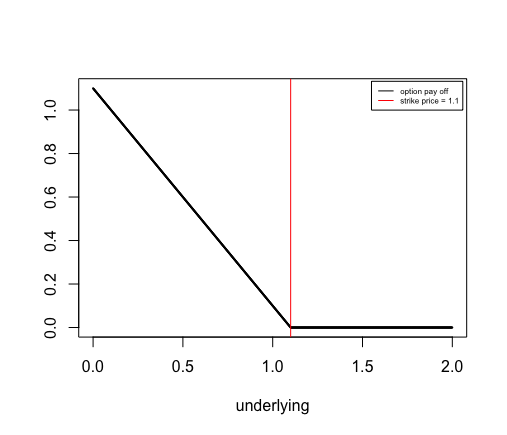
\includegraphics[scale=0.7]{PlotOption.png}
  \label{fig:PlotOption}
  \caption{Auszahlung einer Put Option mit strike 1.1}
\end{figure}

Für eine europäische Option, bei der der Ausübungszeitpunkt bekannt ist, ist die Bewertung der Option mittels Black-Scholes in geschlossener Form möglich. Hierbei wird die Differentialgleichung des Black-Scholes Modells gelöst und unter Zuhilfenahme eines Maßwechsels folgt eine einfache, geschlossene Formel. Diese ist in \cite{Hull} auf S313 zu finden. Weiters führt Hull auch eine Skizze zur Herleitung an.\\
Die Schwierigkeit bei der Berwertung Amerikanischer Optionen besteht darin, dass der Aus-übungszeitpunkt nicht bekannt ist. Der K"aufer der Option muss also zu jedem Zeitpunkt abwägen ob die Option ausgeübt werden sollt, oder ob die Alternative d.h. die Beibehaltung der Option und eine spätere Aus"ubung sinvoller ist. Es wird also in jedem Zeitpunkt der Auszahlungsbetrag bei Aus"ubung und der Erwartungswert bei Beibehaltung verglichen (vgl.  \cite[S.114]{schwartz2001}). Longstaff und Schwartz schätzen diesen bedingten Erwartungswert durch die \glqq fitted values \grqq - also die geschätzten Werte - einer Regression, der Stock prices auf die ex-post Auszahlungen "uber alle Simulationen.


\section{Beispiel}

Folgendes Beispiel soll helfen den Least Squares Monte Carlo (LSM) Algorithmus zu veranschaulichen. In diesem Beispiel soll eine Amerikanische Put-Option (in long position) bewertet werden. Der aktuelle Preis sei normiert und liegt bei 1. Der Strike Preis (i.e. Aus"ubungspreis der Option) bei $K=1.1$. Man gehe weiters davon aus, dass die Option j"ahrlich ausge"ubt werden kann und eine Laufzeit von 4 Jahren hat.\\
Im ersten Schritt werden sog. Pfade simuliert. Hierbei handelt es sich um den Preis des Underlyings. Die Anzahl der Pfade ist dabei beliebig. Um das Beispiel "ubersichtlich zu gestalten werden wir hier nur 10 Pfade simulieren. Jeder Pfad hat die L"ange 4, denn wir simulieren f"ur die gesamte Laufzeit der Option.\\


Tabelle \ref{tab:M} enth"alt die Matrix der Simulationen des Underlyings. Ein Plot der Pfade findet sich in Abbildung \ref{fig:pfade}.





\begin{table}[H] \centering 
  \caption{Simulationsmatrix} 
  \label{tab:M} 
\begin{tabular}{@{\extracolsep{5pt}} cccccc} 
\\[-1.8ex]\hline 
\hline \\[-1.8ex] 
 & t0 & t1 & t2 & t3 & t4 \\ 
\hline \\[-1.8ex] 
1 & $1$ & $0.832$ & $1.199$ & $0.879$ & $1.007$ \\ 
2 & $1$ & $0.931$ & $1.039$ & $0.973$ & $0.885$ \\ 
3 & $1$ & $1.091$ & $1.588$ & $1.280$ & $1.549$ \\ 
4 & $1$ & $1.021$ & $1.054$ & $0.836$ & $1.099$ \\ 
5 & $1$ & $1.039$ & $0.872$ & $0.685$ & $0.931$ \\ 
6 & $1$ & $1.515$ & $2.051$ & $1.545$ & $1.751$ \\ 
7 & $1$ & $1.138$ & $1.288$ & $1.539$ & $1.705$ \\ 
8 & $1$ & $0.620$ & $0.030$ & $0.077$ & $0.058$ \\ 
9 & $1$ & $0.794$ & $1.004$ & $0.663$ & $0.571$ \\ 
10 & $1$ & $0.866$ & $0.724$ & $1.101$ & $0.986$ \\ 
\hline \\[-1.8ex] 
\end{tabular} 
\end{table} 


\begin{figure}[H]

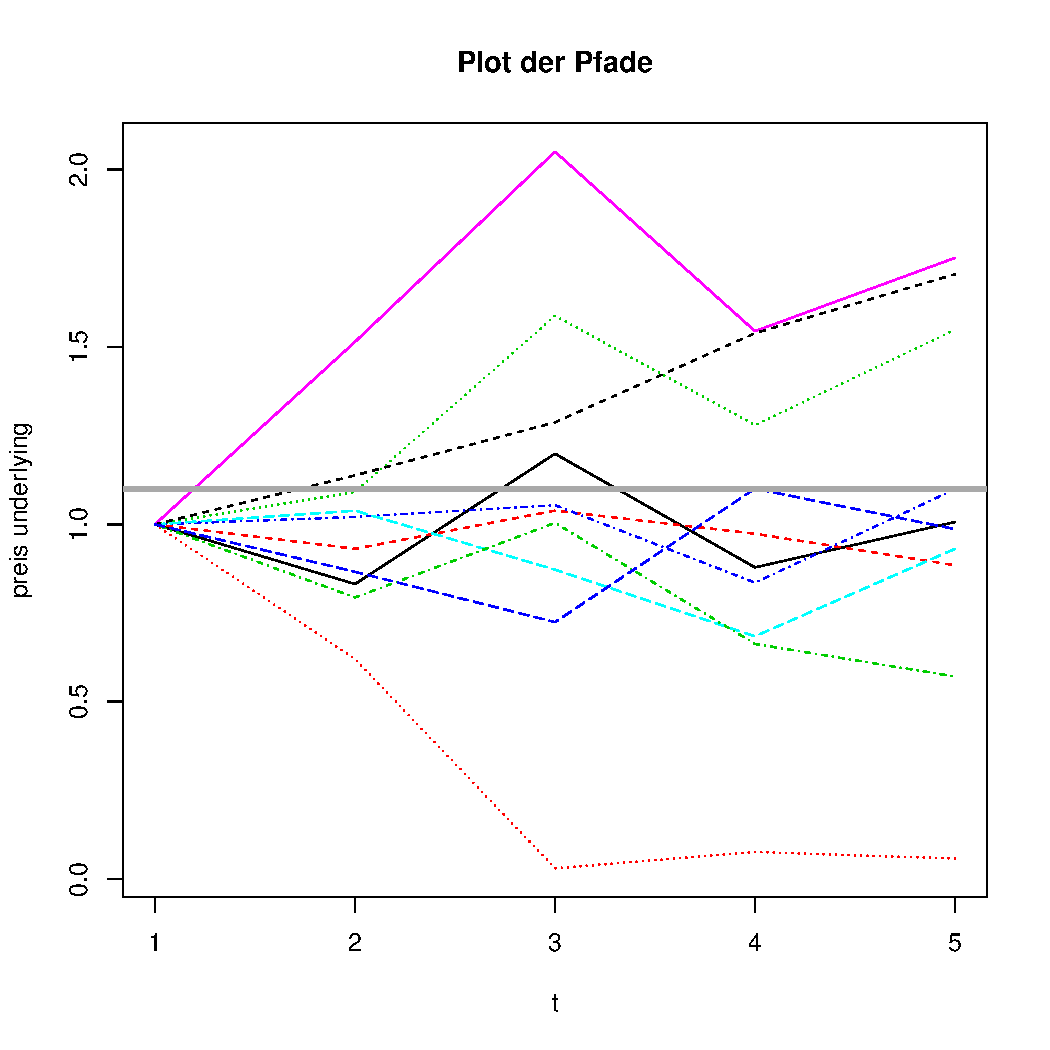
\includegraphics[width=\maxwidth]{figure/unnamed-chunk-3-1} 

\label{fig:pfade}
\caption{Plot der sumulierten 10 Pfade; Strikepreis in grau eingezeichnet}
\end{figure}

LSM ist ein rekursiver Algorithmus \cite[S.116]{schwartz2001}. D.h. wir beginnen die Iterationen mit dem Laufzeitende (hier t=4). Die Auszahlung am Laufzeitende f"ur eine Put Option berechnet sich mit $A_T=max(K-x_T, 0)$ (allgmein $A_t=max(K-x_t, 0)$, wobei $x_t$ der Preis des Underlyings mit $t\in\{1,...,T\}$).


\begin{table}[H] \centering 
  \caption{Auszahlungsmatrix im Zeitpunkt t=4} 
  \label{tab:A} 
\begin{tabular}{@{\extracolsep{5pt}} cccccc} 
\\[-1.8ex]\hline 
\hline \\[-1.8ex] 
 & t0 & t1 & t2 & t3 & t4 \\ 
\hline \\[-1.8ex] 
1 & $$ & $$ & $$ & $$ & $0.093$ \\ 
2 & $$ & $$ & $$ & $$ & $0.215$ \\ 
3 & $$ & $$ & $$ & $$ & $0$ \\ 
4 & $$ & $$ & $$ & $$ & $0.001$ \\ 
5 & $$ & $$ & $$ & $$ & $0.169$ \\ 
6 & $$ & $$ & $$ & $$ & $0$ \\ 
7 & $$ & $$ & $$ & $$ & $0$ \\ 
8 & $$ & $$ & $$ & $$ & $1.042$ \\ 
9 & $$ & $$ & $$ & $$ & $0.529$ \\ 
10 & $$ & $$ & $$ & $$ & $0.114$ \\ 
\hline \\[-1.8ex] 
\end{tabular} 
\end{table} 


Nun gilt es die erwarteten Auszahlungen der Option in $t=4$ zu sch"atzen, ausgehend von den simulierten Preisen des Unterlyings im Zeitpunkt $t=3$. Um den Zeitwert der Auszahlungen zu ber"ucksichtigen wird um eine Periode abgezinst. I.e. die auf den Zeitpunkt t um eine Periode abgezinste Auszahlung $A_t(-1)$ bei einem Zinssatz r berechnet sich aus der Auszahlung $A_t$ wie folgt:  
\[A_t(-1)=A_t*exp(-r)\] 
Um den Erwartungswert in Abh"angigkeit vom Simulierten Underlying zu sch"atzen, verwenden wir folgendes lineares Modell.
\[  y_i=x_i* \beta_1 +x_i^2* \beta_2 +u_i \]
wobei $y_i$ $A_t(-1)$ des jeweiligen Pfades $i=1,...10$ und $x_i$ der Preis des undelyings $x_t$ des jeweiligen Pfades. F"ur den ersten Regressionschritt ist $t=3$ in unserem Beispiel.\\
In der Tabelle \ref{tab:R3} sind die Daten f"ur die Regression zusammengefasst. Es werden nur die Pfade verwendet, bei denen die Option in $t=3$ ausgef"uhrt w"urde, also bei denen es in $t=3$ einen Cash Flow gibt (m.a.W. in the money).


\begin{table}[H] \centering 
  \caption{Datenmatrix zur Regression im ZP t=3} 
  \label{tab:R3} 
\begin{tabular}{@{\extracolsep{5pt}} ccc} 
\\[-1.8ex]\hline 
\hline \\[-1.8ex] 
 & Y & X \\ 
\hline \\[-1.8ex] 
1 & $0.088$ & $0.221$ \\ 
2 & $0.203$ & $0.127$ \\ 
4 & $0.001$ & $0.264$ \\ 
5 & $0.159$ & $0.415$ \\ 
8 & $0.981$ & $1.023$ \\ 
9 & $0.498$ & $0.437$ \\ 
\hline \\[-1.8ex] 
\end{tabular} 
\end{table} 



Wir betrachten nun also die Werte des Sch"atzers $\hat{y_i}=x_i*\hat{\beta_1}+x_i^2*\hat{\beta_2}$ und vergleichen diese mit den Werten, wenn wir die Option in $t=3$ aus"uben w"urden.


\begin{table}[H] \centering 
  \caption{Vergleiche Ausueben vs. Beibehalten im ZP t=3} 
  \label{tab:AB} 
\begin{tabular}{@{\extracolsep{5pt}} ccc} 
\\[-1.8ex]\hline 
\hline \\[-1.8ex] 
 & beibehalten & ausueben \\ 
\hline \\[-1.8ex] 
1 & $0.121$ & $0.221$ \\ 
2 & $0.023$ & $0.127$ \\ 
4 & $0.166$ & $0.264$ \\ 
5 & $0.322$ & $0.415$ \\ 
8 & $0.953$ & $1.023$ \\ 
9 & $0.345$ & $0.437$ \\ 
\hline \\[-1.8ex] 
\end{tabular} 
\end{table} 


Beim Vergleich der Werte in Tabelle \ref{tab:AB} sollte jeweils in t=3 ausge"ubt werden, wenn Aus"uben$>$Beibehalten und umgekehrt. Es f"allt auf, dass zu t=3 in allen Pfaden, die in the money sind (also 1,2,4,5,8 und 9) ausge"ubt werden soll. An diesen Pfaden "ubernehmen wir den Wert in die Auszahlungsmatrix und setzen den Wert in t=4 auf null, weil die Amerikanische Option nur einmal ausge"ubt werden kann.


\begin{table}[H] \centering 
  \caption{Auszahlungsmatrix im Zeitpunkt t=3} 
  \label{tab:A3} 
\begin{tabular}{@{\extracolsep{5pt}} cccccc} 
\\[-1.8ex]\hline 
\hline \\[-1.8ex] 
 & t0 & t1 & t2 & t3 & t4 \\ 
\hline \\[-1.8ex] 
1 & $$ & $$ & $$ & $0.221$ & $0$ \\ 
2 & $$ & $$ & $$ & $0.127$ & $0$ \\ 
3 & $$ & $$ & $$ & $0$ & $0$ \\ 
4 & $$ & $$ & $$ & $0.264$ & $0$ \\ 
5 & $$ & $$ & $$ & $0.415$ & $0$ \\ 
6 & $$ & $$ & $$ & $0$ & $0$ \\ 
7 & $$ & $$ & $$ & $0$ & $0$ \\ 
8 & $$ & $$ & $$ & $1.023$ & $0$ \\ 
9 & $$ & $$ & $$ & $0.437$ & $0$ \\ 
10 & $$ & $$ & $$ & $0$ & $0.114$ \\ 
\hline \\[-1.8ex] 
\end{tabular} 
\end{table} 


Nun modellieren wir eine linieare Regression wie oben mit den Preisen des Underlying zu $t=2$ als X. Y sei der vorausgegangene Wert der Option bei Aus"ubung, abgezinst auf den Zeitpunkt $t$.


\begin{table}[H] \centering 
  \caption{Datenmatrix zur Regression im ZP t=2} 
  \label{tab:R2} 
\begin{tabular}{@{\extracolsep{5pt}} ccc} 
\\[-1.8ex]\hline 
\hline \\[-1.8ex] 
 & Y & X \\ 
\hline \\[-1.8ex] 
2 & $0.119$ & $0.061$ \\ 
4 & $0.249$ & $0.046$ \\ 
5 & $0.391$ & $0.228$ \\ 
8 & $0.964$ & $1.070$ \\ 
9 & $0.412$ & $0.096$ \\ 
10 & $0.101$ & $0.376$ \\ 
\hline \\[-1.8ex] 
\end{tabular} 
\end{table} 

\begin{table}[H] \centering 
  \caption{Vergleiche Ausueben vs. Beibehalten im ZP t=2} 
  \label{tab:AB2} 
\begin{tabular}{@{\extracolsep{5pt}} ccc} 
\\[-1.8ex]\hline 
\hline \\[-1.8ex] 
 & beibehalten & ausueben \\ 
\hline \\[-1.8ex] 
2 & $0.203$ & $0.061$ \\ 
4 & $0.192$ & $0.046$ \\ 
5 & $0.315$ & $0.228$ \\ 
8 & $0.884$ & $1.070$ \\ 
9 & $0.226$ & $0.096$ \\ 
10 & $0.415$ & $0.376$ \\ 
\hline \\[-1.8ex] 
\end{tabular} 
\end{table} 


Im ZP t=2 wird nur im den Pfad 8 ausge"ubt, ansonsten wird beibahalten. Das f"uhrt zur Auszahlungsmatrix Tabelle \ref{tab:A2}.


\begin{table}[H] \centering 
  \caption{Auszahlungsmatrix im Zeitpunkt t=2} 
  \label{tab:A2} 
\begin{tabular}{@{\extracolsep{5pt}} cccccc} 
\\[-1.8ex]\hline 
\hline \\[-1.8ex] 
 & t0 & t1 & t2 & t3 & t4 \\ 
\hline \\[-1.8ex] 
1 & $$ & $$ & $0$ & $0.221$ & $0$ \\ 
2 & $$ & $$ & $0$ & $0.127$ & $0$ \\ 
3 & $$ & $$ & $0$ & $0$ & $0$ \\ 
4 & $$ & $$ & $0$ & $0.264$ & $0$ \\ 
5 & $$ & $$ & $0$ & $0.415$ & $0$ \\ 
6 & $$ & $$ & $0$ & $0$ & $0$ \\ 
7 & $$ & $$ & $0$ & $0$ & $0$ \\ 
8 & $$ & $$ & $1.070$ & $0$ & $0$ \\ 
9 & $$ & $$ & $0$ & $0.437$ & $0$ \\ 
10 & $$ & $$ & $0$ & $0$ & $0.114$ \\ 
\hline \\[-1.8ex] 
\end{tabular} 
\end{table} 


F"ur den letzten Schritt t=1 verfahren wir genauso.


\begin{table}[H] \centering 
  \caption{Auszahlungsmatrix im Zeitpunkt t=1} 
  \label{tab:A1} 
\begin{tabular}{@{\extracolsep{5pt}} cccccc} 
\\[-1.8ex]\hline 
\hline \\[-1.8ex] 
 & t0 & t1 & t2 & t3 & t4 \\ 
\hline \\[-1.8ex] 
1 & $$ & $0$ & $0$ & $0.221$ & $0$ \\ 
2 & $$ & $0$ & $0$ & $0.127$ & $0$ \\ 
3 & $$ & $0.009$ & $0$ & $0$ & $0$ \\ 
4 & $$ & $0$ & $0$ & $0.264$ & $0$ \\ 
5 & $$ & $0$ & $0$ & $0.415$ & $0$ \\ 
6 & $$ & $0$ & $0$ & $0$ & $0$ \\ 
7 & $$ & $0$ & $0$ & $0$ & $0$ \\ 
8 & $$ & $0$ & $1.070$ & $0$ & $0$ \\ 
9 & $$ & $0$ & $0$ & $0.437$ & $0$ \\ 
10 & $$ & $0$ & $0$ & $0$ & $0.114$ \\ 
\hline \\[-1.8ex] 
\end{tabular} 
\end{table} 


Im ZP t=0 kann die Option nicht ausge"ubt werden, deswegen ist t=0 irrelevant. Die Auszahlungen der Option werden jeweils auf den Zeitpunkt t=0 diskontiert.


\begin{table}[H] \centering 
  \caption{Diskontierte Auszahlungsmatrix} 
  \label{tab:A1} 
\begin{tabular}{@{\extracolsep{5pt}} ccccc} 
\\[-1.8ex]\hline 
\hline \\[-1.8ex] 
 & t1 & t2 & t3 & t4 \\ 
\hline \\[-1.8ex] 
1 & $0$ & $0$ & $0.185$ & $0$ \\ 
2 & $0$ & $0$ & $0.106$ & $0$ \\ 
3 & $0.008$ & $0$ & $0$ & $0$ \\ 
4 & $0$ & $0$ & $0.221$ & $0$ \\ 
5 & $0$ & $0$ & $0.347$ & $0$ \\ 
6 & $0$ & $0$ & $0$ & $0$ \\ 
7 & $0$ & $0$ & $0$ & $0$ \\ 
8 & $0$ & $0.949$ & $0$ & $0$ \\ 
9 & $0$ & $0$ & $0.365$ & $0$ \\ 
10 & $0$ & $0$ & $0$ & $0.089$ \\ 
\hline \\[-1.8ex] 
\end{tabular} 
\end{table} 


Der Preis der Option berechnet sich durch Mitteln der diskontierten Auszahlungen.
In diesem Beispiel:
0.173

\chapter{Anwendung}

Angenommen man möchte nun LSM auf eine amerikanische Put Option anwenden. Zum Stock (dem Underlying der Option) sei der Mittelwert und die Varianz bekannt. Wir gehen in diesem Fall von einer Laufzeit von einem Jahr und einem strike price von 1.1 aus. Innerhalb dieses Jahres, kann die Option zu jedem Handelstag ausgeübt werden. 
Zur Bepreisung dieser Option müssen wir nun in einem ersten Schritt ausreichend viele Trajektorien über den Zeitraum der Laufzeit hinweg simulieren. Dann, lässt sich LSM auf diese Simulation anweden. 

Bemerkung: LSM ist eine Heuristik ausschließlich gedacht zur Ermittlung eines fairen Preises einer Option, nicht zur Berechnung des optimalen Ausübungszeitpunktes.

\section{Simulation via Black-Scholes}

F"ur diese Arbeit sollen die Preise anhand des Black-Scholes Modells Stockpreise für ein Jahr simuliert werden. Man gehe von einem B"orsenjahr aus. D.h. für 2019: 252 Handelstage \cite[]{boersewien2019}.\\
Man gehe davon aus, dass ein Stock zum ersten B"orsentag mit dem Preis $S_0$ startet. Hier sei $S_0=1$. Der risikofreie Zinssatz $r$ betrage 1\%. Der Wiener Prozess zur Simulation der Black Scholes Stock Preise sei mit dem Parameter $\mu=0$ für alle Trajektorien spezifiziert. Für jede Trajektorie sind die Parameter $\sigma$ und $\mu$ des Wiener Prozess gleich und stammen von den geschätzten Parametern des stocks (i.e. $\sigma \equiv \sqrt{\hat{\sigma^2}}$ ... Schätzer für Volatilität und $\mu \equiv \hat{\mu}$ ... Schätzer für den Drift). Damit ergibt sich ein Prozess mit Martingaleigenschaft:

$$S^*(t)=S_0 exp\left\{  (r-\frac{\sigma^2}{2})t + \sigma W_t\right\}$$

Wobei $W_t$ ein Wiener Prozess mit Drift $\mu$ und Varianz $\sigma^2$ ist.

In der Abbildung \ref{fig:pfade252} ist exemplarisch ein Plot mit 15 Pfaden angeführt.


\begin{figure}[H]

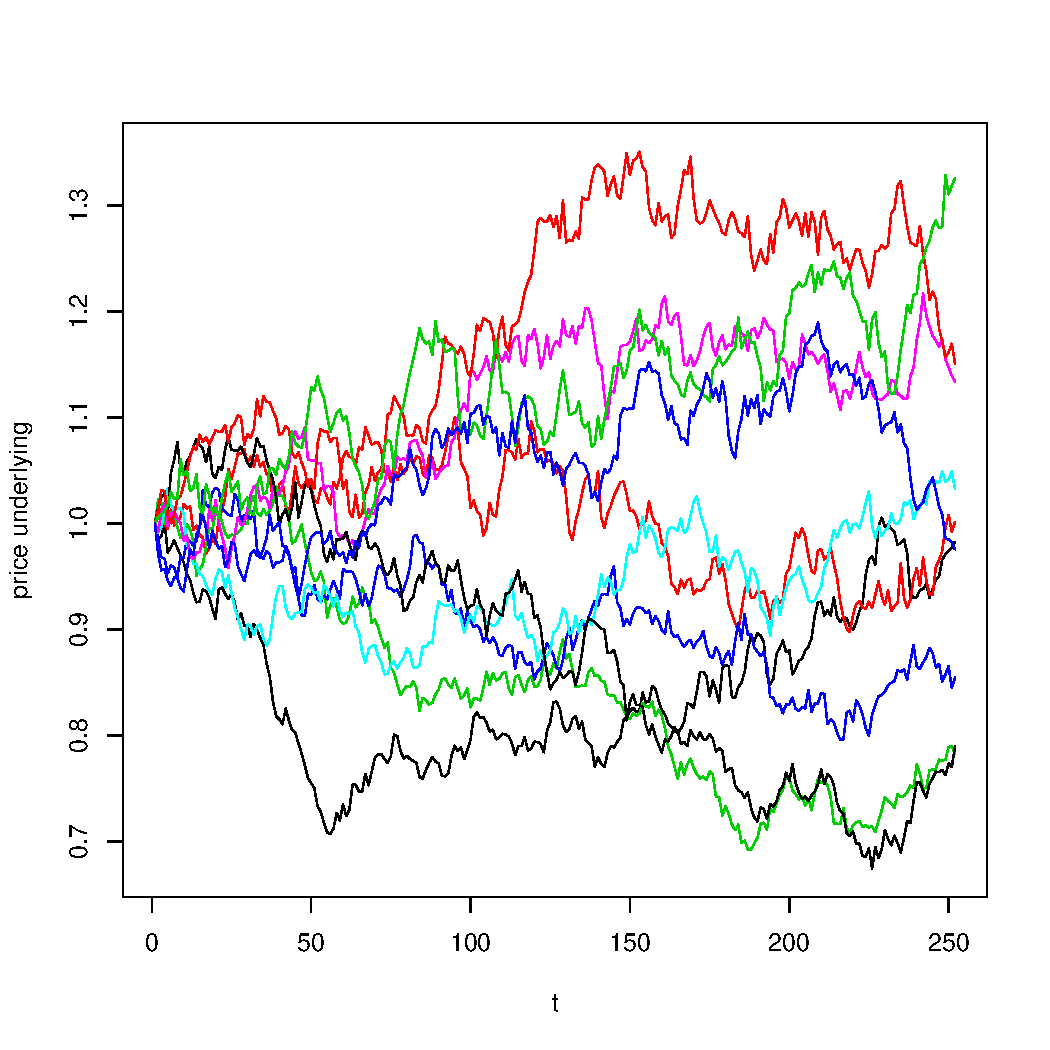
\includegraphics[width=\maxwidth]{figure/unnamed-chunk-14-1} 

\caption{Plot einer Simulation von 15 Pfaden "uber 252 Tage}
\label{fig:pfade252}
\end{figure}

Es soll überprüft werden, ob der simulierte Prozess tatsächlich ein Martingal darstellt. Angenommen ein Prozess $(X_t)_{t\geq 1}$ sei integrierbar und adaptiert (d.h. $\mathcal{F}_n$ meßbar f"ur alle $n \in \mathbb{N}$, wobei $\mathcal{F}_n$ eine Filtration zum ZP $n$). Dann ist der Prozess ein Martingal wenn er die folgende Martingaleigenschaft erfüllt:
\[ \mathbb{E}[X_{t+1}| \mathcal{F}_t]=X_t \ \ f.s.\ \ \forall t \in \mathbb{N}\]
Für unseren simulierten Fall würde das bedeuten, dass der Prozess einen konstanten, diskontierten Erwartungswert hat, was es zu "uberpr"ufen gilt. Im Folgenden wird also der Erwartungswert für alle $t$ durch das arithmetische Mittel geschätzt. Um validere Ergebnisse zu erhalten sollen nun 1000 Pfade simuliert werden (Plot im Appendix Abbildung \ref{100P}). Der Plot in Abbildung \ref{EWfig} zeigt die Sch"atzer für alle Beobachtungen. 

\begin{figure}[H]

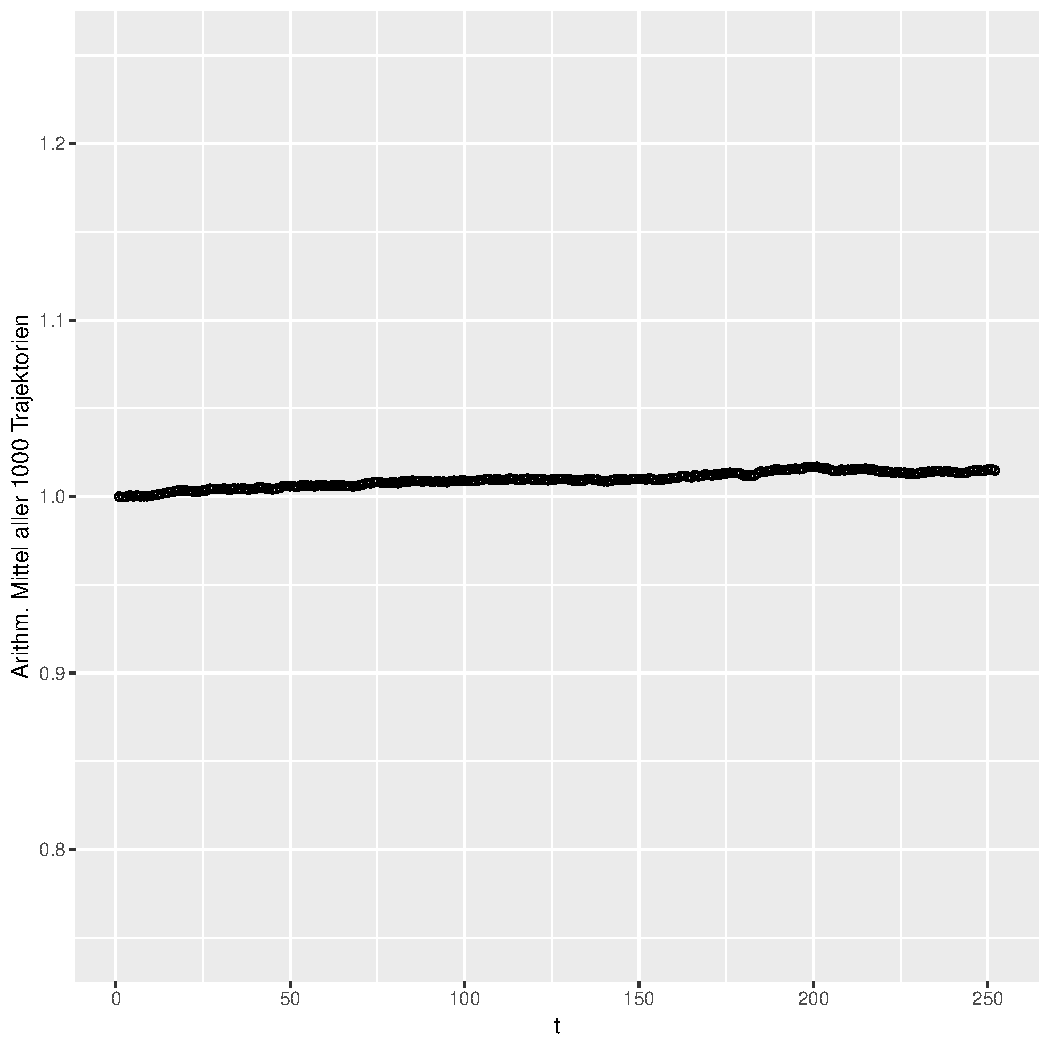
\includegraphics[width=\maxwidth]{figure/unnamed-chunk-15-1} 

\caption{Plot der gesch"atzten Erwartungswerte (d.h. arithm. Mittel) für den Prozess mit 1000 Pfaden}
\label{EWfig}
\end{figure}

Der Plot der Mittel in Abbildung \ref{EWfig} st"utzt die Annahme, dass der Erwartungswert für alle $t \in \mathbb{N}$ konstant ist. Man kann also davon ausgehen, dass es sich bei dem simulierten Prozess um ein Martingal handelt. 

\section{Anwendung von LSM auf simulierte Preise}

Nun wollen wir LSM auf die simulierten Preise anweden um einen fairen Preis für die Option zu berechnen. Dazu soll die Funktion \textit{LSM()} (s. Appendix) dienen, die die simulierte Matrix als Argument übernimmt. 


\ \\
Der gemittelte Ertrag pro Ausübung beträgt nach LSM 
0.129

\ \\
Wir haben im einführenden Beispiel und für den LSM Algorithmus oben ein Polynom 2. Grades für das lineare Modell gewählt. Nun stellt sich die Frage: wie unterschiedlich sind die Ergebnisse für verschiedene Modelle?\\
Weil es diese Arbeit im Umfang nicht zulässt alle möglichen Modelle zu evaluieren, möchte ich im Folgenden nur eine Übersicht über einige wenige ALternativen geben. Interessant ist möglicherweise der Vergleich zu einem einfachen linearen Modell ohne Transformation, einem linearen Modell mit einer Transformation zu einem Polynom dritten Grades, und eines mit einem Polynom 10ten Grades. 

Bemerkung: Diese Modelle sind willkürlich gewählt und sollen dem Leser nur einen Überblick vermitteln.





% Table created by stargazer v.5.2.2 by Marek Hlavac, Harvard University. E-mail: hlavac at fas.harvard.edu
% Date and time: Mi, Mär 20, 2019 - 14:58:41
\begin{table}[!htbp] \centering 
  \caption{} 
  \label{} 
\begin{tabular}{@{\extracolsep{5pt}} ccc} 
\\[-1.8ex]\hline 
\hline \\[-1.8ex] 
 & Modell & Optionspreis \\ 
\hline \\[-1.8ex] 
1 & einfach & $0.128830$ \\ 
2 & Polynom 2 & $0.128830$ \\ 
3 & Polynom 3 & $0.128830$ \\ 
4 & Polynom 10 & $0.128830$ \\ 
\hline \\[-1.8ex] 
\end{tabular} 
\end{table} 


Wir beobachten, dass die Optionspreise ident sind. Es ist nicht mit Sicherheit zu sagen, woran das liegt, aber es liegt nahe, dass die Information der simulierten Werte ausreicht, um selbst mit dem einfachen linearen Modell an den selben Zeitpunkten entscheidet auszuüben, wie auch bei den koplexeren Modellen.

\bibliography{SeminararbeitBiBTex}
\bibliographystyle{apalike}


\appendix

\chapter*{Appendix}

\begin{figure}[H]

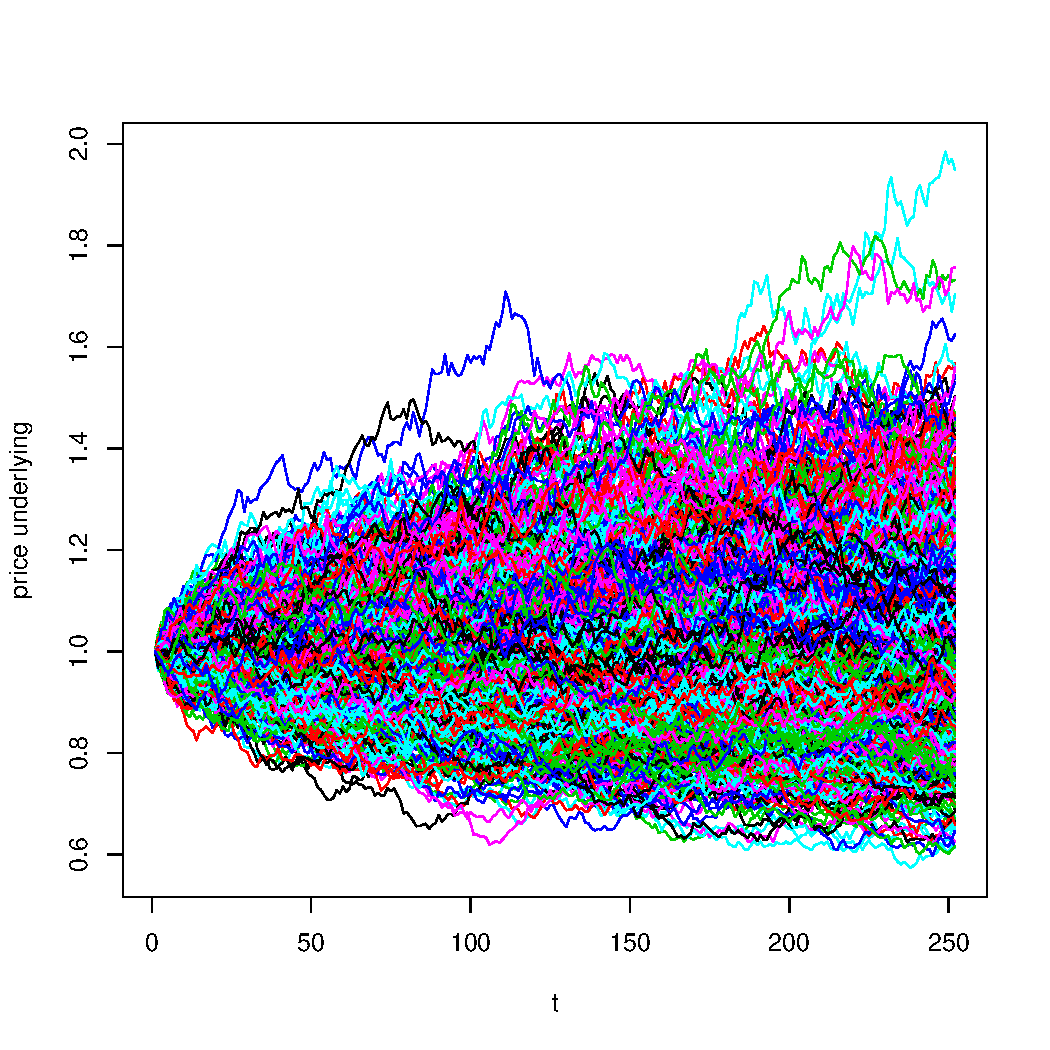
\includegraphics[width=\maxwidth]{figure/unnamed-chunk-20-1} 

\caption{Plot der Simulation mit 1000 Pfaden}
\label{100P}
\end{figure}

Funktion \textit{simMatrix()} um die Matrix der stock Preise zu simulieren.

\begin{kframe}
\begin{alltt}
\hlstd{simMatrix} \hlkwb{<-} \hlkwa{function}\hlstd{(}\hlkwc{S0}\hlstd{=}\hlnum{100}\hlstd{,} \hlkwc{Nsimulations}\hlstd{=}\hlnum{100}\hlstd{,} \hlkwc{r}\hlstd{=}\hlnum{0.01}\hlstd{,}
                      \hlkwc{sigma}\hlstd{=}\hlnum{0.2}\hlstd{,} \hlkwc{se}\hlstd{=}\hlnum{123}\hlstd{)\{}
  \hlcom{# simMatrix is a function, simulating a Matrix of stock}
  \hlcom{# prices for one year. The number of simulations can be}
  \hlcom{# set by the parameter Nsimulations. }
  \hlcom{# The function simulates the Stock prices using the }
  \hlcom{# Black-Scholes Model. The Stock price for t>0 is given}
  \hlcom{# by: S_t = S_0 * exp\{r-sigma^2/2)*t + sigma*W_t\}, where W_t is }
  \hlcom{# a Brownian Motion with mu=0 and variance is the time increment.}
  \hlcom{# Nsimulations ... Number of simulations (int)}
  \hlcom{# S0 ............. Starting value (int)}
  \hlcom{# r .............. risk free interest rate (int)}
  \hlcom{# sigma .......... the parameter sigma for the Black Scholes}
  \hlcom{#                  simulation. }
  \hlcom{# se ............. set seed (int)}

  \hlkwd{set.seed}\hlstd{(se)}
  \hlstd{M} \hlkwb{<-} \hlkwd{matrix}\hlstd{(}\hlnum{NA}\hlstd{,} \hlkwc{nrow}\hlstd{=Nsimulations,} \hlkwc{ncol}\hlstd{=}\hlnum{252}\hlstd{)}
  \hlstd{N} \hlkwb{<-} \hlnum{252}
  \hlkwa{for} \hlstd{(i} \hlkwa{in} \hlnum{1}\hlopt{:}\hlstd{Nsimulations)\{}

    \hlcom{# Brownian Motion}
    \hlstd{m} \hlkwb{<-} \hlnum{0}
    \hlstd{dW} \hlkwb{<-} \hlkwd{rnorm}\hlstd{(}\hlkwc{n}\hlstd{=N,} \hlkwc{mean}\hlstd{=m,} \hlkwc{sd}\hlstd{=}\hlkwd{sqrt}\hlstd{(}\hlnum{1}\hlopt{/}\hlnum{252}\hlstd{))}
    \hlstd{W} \hlkwb{<-} \hlkwd{c}\hlstd{(}\hlnum{0}\hlstd{,} \hlkwd{cumsum}\hlstd{(dW))}

    \hlstd{t} \hlkwb{<-} \hlnum{1}\hlopt{:}\hlstd{N}
    \hlstd{S} \hlkwb{<-} \hlstd{S0}\hlopt{*}\hlkwd{exp}\hlstd{((r}\hlopt{-}\hlstd{(sigma}\hlopt{^}\hlnum{2}\hlstd{)}\hlopt{/}\hlnum{2}\hlstd{)}\hlopt{*}\hlstd{(t}\hlopt{/}\hlnum{252}\hlstd{)}\hlopt{+}\hlstd{sigma}\hlopt{*}\hlstd{W[t])}
    \hlstd{M[i,]} \hlkwb{<-} \hlstd{S}
  \hlstd{\}}
  \hlkwd{colnames}\hlstd{(M)} \hlkwb{<-} \hlnum{1}\hlopt{:}\hlnum{252}
  \hlkwd{rownames}\hlstd{(M)} \hlkwb{<-} \hlkwd{paste}\hlstd{(}\hlstr{"sim"}\hlstd{,} \hlnum{1}\hlopt{:}\hlstd{Nsimulations)}
  \hlkwd{return}\hlstd{(M)}
\hlstd{\}}
\end{alltt}
\end{kframe}

Funktion \textit{LSM} um ein LSM Algoritmus auf die Simulation anzuwenden.

\begin{kframe}
\begin{alltt}
\hlstd{LSM} \hlkwb{<-} \hlkwa{function}\hlstd{(}\hlkwc{M}\hlstd{,} \hlkwc{K}\hlstd{=}\hlnum{1.1}\hlstd{,} \hlkwc{r}\hlstd{=}\hlnum{0.06}\hlstd{)\{}
  \hlcom{# This function performs the Least Squares Monte Carlo}
  \hlcom{# algorithm for any simulated matrix M. The output}
  \hlcom{# is the mean of the discounted cash flow of returns }
  \hlcom{# where the option was exercised.}
  \hlcom{# M ... simulated matrix}
  \hlcom{# K ... strike price}
  \hlcom{# r ... interest rate}
  \hlstd{T} \hlkwb{<-} \hlkwd{ncol}\hlstd{(M)}
  \hlstd{t} \hlkwb{<-} \hlstd{T}\hlopt{-}\hlnum{1}
  \hlstd{N} \hlkwb{<-} \hlkwd{nrow}\hlstd{(M)}
  \hlstd{Ai} \hlkwb{<-} \hlkwd{matrix}\hlstd{(}\hlnum{0}\hlstd{,} \hlkwc{nrow}\hlstd{=N,} \hlkwc{ncol}\hlstd{=T)}
  \hlkwd{lapply}\hlstd{(M[,t}\hlopt{+}\hlnum{1}\hlstd{],}\hlkwa{function}\hlstd{(}\hlkwc{x}\hlstd{)} \hlkwd{max}\hlstd{(K}\hlopt{-}\hlstd{x,}\hlnum{0}\hlstd{))}  \hlopt \hlstd{unlist} \hlkwb{->} \hlstd{Ai[,t}\hlopt{+}\hlnum{1}\hlstd{]}

  \hlkwa{for} \hlstd{(t} \hlkwa{in} \hlstd{(T}\hlopt{-}\hlnum{1}\hlstd{)}\hlopt{:}\hlnum{2}\hlstd{)\{}
    \hlkwd{lapply}\hlstd{(M[,t],}\hlkwa{function}\hlstd{(}\hlkwc{x}\hlstd{)} \hlkwd{max}\hlstd{(K}\hlopt{-}\hlstd{x,}\hlnum{0}\hlstd{))}  \hlopt \hlstd{unlist} \hlopt
      \hlkwd{Filter}\hlstd{(}\hlkwc{f}\hlstd{=}\hlkwa{function}\hlstd{(}\hlkwc{x}\hlstd{) x}\hlopt{!=}\hlnum{0}\hlstd{)}\hlkwb{->} \hlstd{im}
    \hlkwd{names}\hlstd{(im)} \hlopt \hlkwd{as.numeric}\hlstd{()} \hlkwb{->} \hlstd{ind}
    \hlcom{# discounting}
    \hlstd{Y} \hlkwb{<-} \hlkwd{rep}\hlstd{(}\hlnum{0}\hlstd{,}\hlkwd{length}\hlstd{(ind))}
    \hlkwa{for} \hlstd{(i} \hlkwa{in} \hlnum{1}\hlopt{:}\hlstd{(T}\hlopt{-}\hlstd{t))\{}
      \hlstd{Y} \hlkwb{<-} \hlstd{Y}\hlopt{+}\hlkwd{exp}\hlstd{(}\hlopt{-}\hlstd{r}\hlopt{*}\hlstd{i)}\hlopt{*}\hlstd{Ai[ind,t}\hlopt{+}\hlstd{i]}
    \hlstd{\}}
    \hlstd{X} \hlkwb{<-} \hlstd{im}
    \hlstd{lm1} \hlkwb{<-} \hlkwd{lm}\hlstd{(Y}\hlopt{~}\hlstd{X}\hlopt{+}\hlstd{(X}\hlopt{^}\hlnum{2}\hlstd{))}
    \hlstd{f1} \hlkwb{<-} \hlstd{lm1}\hlopt{$}\hlstd{fitted.values}
    \hlcom{# exercise vs keep}
    \hlstd{df} \hlkwb{<-} \hlkwd{data.frame}\hlstd{(}\hlkwc{beibehalten}\hlstd{=f1,} \hlkwc{ausueben}\hlstd{=im)}
    \hlstd{ind2} \hlkwb{<-} \hlkwd{apply}\hlstd{(df,}\hlnum{1}\hlstd{,} \hlkwa{function}\hlstd{(}\hlkwc{x}\hlstd{)} \hlkwd{ifelse}\hlstd{(x[}\hlnum{2}\hlstd{]}\hlopt{>}\hlstd{x[}\hlnum{1}\hlstd{], x[}\hlnum{2}\hlstd{],} \hlnum{0}\hlstd{))}
    \hlstd{Ai[ind,t]} \hlkwb{<-} \hlstd{ind2}
    \hlcom{# set all following to 0}
    \hlstd{Ai[Ai[,t]}\hlopt{!=}\hlnum{0}\hlstd{,(t}\hlopt{+}\hlnum{1}\hlstd{)}\hlopt{:}\hlstd{T]} \hlkwb{<-} \hlnum{0}
  \hlstd{\}}

  \hlstd{Ai} \hlkwb{<-} \hlstd{Ai[,}\hlnum{2}\hlopt{:}\hlstd{T]}
  \hlstd{Y} \hlkwb{<-} \hlkwd{rep}\hlstd{(}\hlnum{0}\hlstd{,N)}
  \hlkwa{for} \hlstd{(i} \hlkwa{in} \hlnum{1}\hlopt{:}\hlstd{(T}\hlopt{-}\hlnum{1}\hlstd{))\{}
    \hlstd{Y} \hlkwb{<-} \hlstd{Y}\hlopt{+}\hlkwd{exp}\hlstd{(}\hlopt{-}\hlstd{r}\hlopt{*}\hlstd{i)}\hlopt{*}\hlstd{Ai[,i]}
  \hlstd{\}}
  \hlkwd{return}\hlstd{(}\hlkwd{mean}\hlstd{(Y))}
\hlstd{\}}
\end{alltt}
\end{kframe}


\end{document}
